\documentclass[../598comp.tex]{subfiles}

\graphicspath{ {./lectures/images/}{./images/} }

\date{05-25}

\begin{document}

\section{05-25}

\subsection{Reductions}

$P$ reduces to $Q$ means if I can solve $Q$ I can solve $P$. This is roughly
equivalent to $Q$ is ``harder than'' $P$.

Algorithm for solving $P$. First transform the problem into a $Q$ problem. Then
feed the problem to the $Q$ solver.

If you \ul{know} $P$ is undecidable than the \ul{putative} $Q$ solver cannot
exist, so $Q$ is also undecidable.

$\leq$ is a preorder. Transitive so reductions can be chained. Not partial order
because it doesn't have anti-symmetry.

Notation. $\langle M \rangle$ is encoding of a machine. $\langle M, w \rangle$
is a machine and its input. $\langle M_1, M_2 \rangle$ is two machines. $\langle
G \rangle$ encodes a CFG.
\begin{align*}
  H_{TM} &= \{\langle M, w \rangle \mid M \ \text{halts on} \ w\} \\
  A_{TM} &= \{\langle M, w \rangle \mid M \ \text{accepts} \ w\}
\end{align*}
$H_{TM}$ accepts the set of machines and input that halt. $A_{TM}$ accepts the
set of machines and inputs that those machines accept. $H_{TM} \leq A_{TM}$.

\begin{note}
  Constructing a machine should be thought of as writing the code for the machine.
\end{note}

Algorithm for $A_{TM}$ cannot exist because $H_{TM}$ reduces to it.

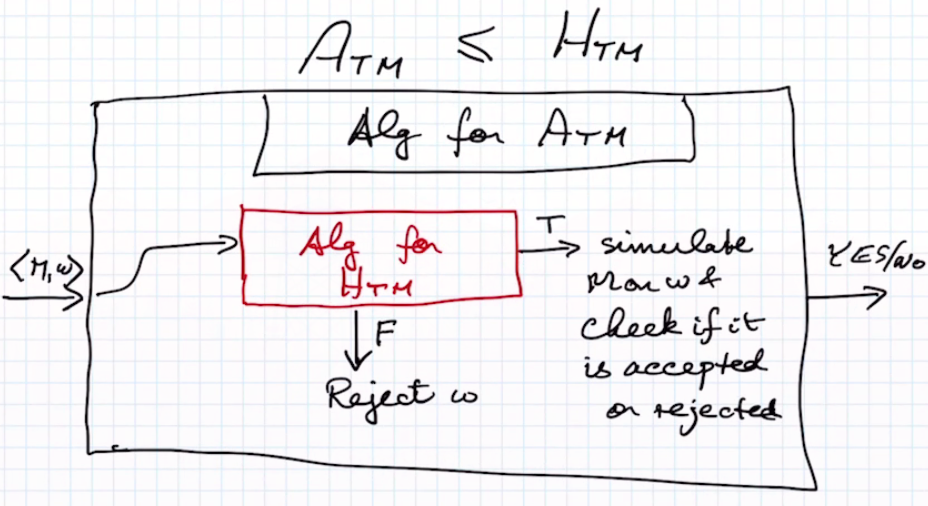
\includegraphics[width=\textwidth]{atm_to_htm_example}

$EMPTY_{TM} = \{\langle M \rangle \mid L(M) = \varnothing\}$.

$A_{TM} \leq EMPTY_{TM}$. Machine:

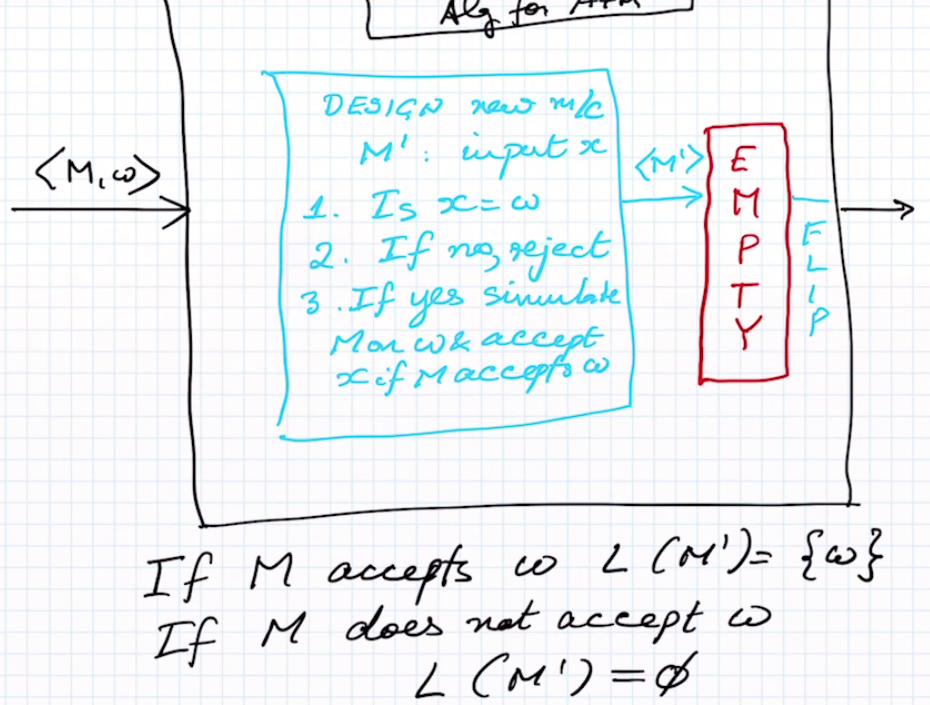
\includegraphics[width=\textwidth]{algorithm_for_empty}

REG, is $L(M)$ a regular language? Construct machine. % review

\begin{note}
  The more powerful a gadget is, the easier it is to build a reduction to that gadget.
\end{note}

$EQ_{TM} = \{\langle M_1, M_2 \rangle \mid L(M_1) = L(M_2)\}$. $EMPTY_{TM} \leq
EQ_{TM}$. Construct a machine that rejects all words, and compare equality of
input to $EMPTY$ with this machine using $EQ$ machine. If they are equal, then
$M$ is empty.

\begin{exercise}
  Show that the following are undecideable.
  \begin{enumerate}
  \item 
    $L(M) = L(M')$ where $M'$ always halts.
  \item
    $L(M)$ is context free.
  \item
    $|L(M)| < \infty$. 
  \item
    $L(M) = \Sigma^*$.
  \end{enumerate}
\end{exercise}

\subsection{Sharper Notion of Reduction}

Mapping reduction. Suppose $L_1, L_2 \subseteq \Sigma^*$. We say $L_1$ is
mapping reducible to $L_2$
\begin{gather*}
  L_1 \leq_m L_2
\end{gather*}
if \ul{there exists} a \ul{total computable} function $f: \Sigma^* \to
\Sigma^*$ such that $\forall w \in \Sigma^*, \ w \in L_1 \iff f(w) \in L_2$.

\begin{note}
  \begin{enumerate}
  \item[]
  \item 
    $L_1 \leq_m L_2$ then $\ol{L_1} \leq_m \ol{L_2}$. This is not true for general reductions.
  \item
    $\leq_m$ has a \ul{direction} because $f$ has a direction. No guarantee that
    you can go both ways. $L_1 \leq_m L_2$ does not mean $L_2 \leq_m L_1$.
  \end{enumerate}
\end{note}

\begin{fact}
  Facts about $\leq_m$.
  \begin{enumerate}
  \item 
    $P \leq_m Q$ and $P$ is undecidable then $Q$ is undecidable
  \item
    $P \leq_m Q$ and $Q$ is decidable then $P$ is decidable.
  \item
    $P \leq_m Q$ and $Q$ is computably enumerable then $P$ is also computably enumerable.
  \item
    $P \leq_m Q$ and $P$ is not computably enumerable, then $Q$ cannot be
    computably enumerable.
  \item
    If $P \leq_m Q$ and $P$ is not co-CE then $Q$ cannot be co-CE. co-CE means
    if the algorithm is NO your algorithm will definitely tell you. CE means if
    the answer is YES your algorithm will definitely tell you.

    $H_{TM}, A_{TM}$ are CE but not coCE. Run it and it will tell you if the
    answer is yes.

    $\ol{A_{TM}}, EMPTY_{TM}$ are co-CE. You will definitely find out if it is
    not empty with dove tailing.
  \end{enumerate}
\end{fact}
Semi decision problem, computably enumerable set.

$A_{TM} \leq EMPTY_{TM}$ but this is not a mapping reduction. Suppose we had
$A_{TM} \leq_m EMPTY_{TM}$, then $\ol{A_{TM}} \leq_m \ol{EMPTY_{TM}}$. But this
is not possible because $\ol{A_{TM}}$ is co-CE while $\ol{EMPTY_{TM}}$ is CE.

\subsection{Turing Reduction}

$P \leq_T Q$. I get to use a $Q$ \ul{oracle} as many times as I want and I can
do any computable post processing I want.

$P \leq_m Q$. I get to do some total computable preprocessing and then ask my
$Q$ oracle 1 question and output the answer without post processing. Can't even
flip the output.

\begin{theorem}
  $EQ_{TM}$ is not CE or coCE. More difficult than halting problem.
\end{theorem}
\begin{fact}
  Halting problem is complete for all CE problems. CE complete.

  Non-halting problem is coCE complete.
\end{fact}

$|L(M)| = \infty$. INF = $\{\langle M \rangle \mid |L(M)| = \infty\}$

Claim: $\ol{H_{TM}} \leq_m INF$.

Reducing of non halting problem. Let input to $M'$ be $X$, then run $M$ on $w$ $|x|$
times and reject $x$ if it halts, accept otherwise. The language of $M'$ is
everything if $w$ runs forever and is finite otherwise, which can be checked
with INF.

\begin{theorem}[Rice's Theorem]
  $P: \NN \to \NN$. $\llbracket P \rrbracket := \{(x, y) \mid P(x) = y\}$.

  $P_1 \sim P_2$ means $\llbracket P_1 \rrbracket = \llbracket P_2 \rrbracket$.

  $P_1, P_2$ are \ul{extensionally equal}.

  $M_1 \sim M_2 \iff L(M_1) = L(M_2)$. $Q: PROG \to \{T, F\}$ is called a
  \ul{property} of programs. $Q$ is an extensional property if $P_1 \sim P_2
  \iff Q(P_1) = Q(P_2)$. $Q$ only depends on the IO behavior. $Q$ only depends
  on the functional spec.

  $Q$ always true or $Q$ always false are trivial properties.

  Rice's theorem: Every non trivial extensional property of programs is
  undecidable. Nothing that just depends on the IO spec can possibly be decidable.
  \begin{proof}
    Let $Q$ be a nontrivial property of CE sets. i.e. $\exists P$ such that
    $Q(P) = true$ and $\exists P'$ such that $Q(P')= false$.

    Assume empty does not satisfy $Q$. i.e. $\forall M$ if $L(M) = \varnothing$
    then $Q(M) = F$.

    Let $M_0$ be such that $Q(M_0) = T$. Then $L(M_0) \neq \varnothing$ by our assumption.
    \begin{gather*}
      L_q = \{\langle M \rangle \mid Q(M) = T\}
    \end{gather*}
    Claim: $A_{TM} \leq_m L_Q$. Have gadget to solve $x \in L_Q$.

    $M'$ with input $x$ construction: Simulate $M$ on $w$. If $M$ accepts $w$
    then simulate $M_0$ on $x$.
  \end{proof}
\end{theorem}


\end{document}

